\documentclass[../../Matt_Gebert_Honours_Thesis.tex]{subfiles}

\begin{document}
	
	To measure the electrical properties of graphene devices (such as those detailed in \cref{sec:fabrication}), particular equipment and methods are employed to observe relevant properties. 
	
	\subsection{4 probe measurements}
	4 probe measurements, also known as Kelvin sensing, utilise four probes to make a more accurate measurement than regular two probe measurements. 
	
	Conventional multimeters use a probing voltage with a galvanometer to detect a current running through a sample (in this case, graphene). Based off the detected current, a measurement can be made of the resistance for the known voltage. Because exfoliated graphene can have very small channel widths, it is very sensitiviy to large currents and consequently makes using a multimeter dangerous. Using a multimeter would be fine however, for large area CVD graphene.
	
	One advantage of using a 4 probe measurement is that you can use a current-limiting resistance, which has a much larger resistance than your sample ($>100\times$). This allows control of the current running through your sample, ensuring safe limits, and means the resistance of your sample will affect the current flow to less than 1\%. By observing the voltage difference across the sample, a resistance can be inferred from the flowing current. Typical exfoliated graphene devices used in this project have a measured resistance on the order of $\approx$5 K$\Omega$ (\cref{eqn:resistance_measurement}).
	
	However, the most significant advantage of using a 4 probe measurement is the ability to avoid including contact resistance, created by the junctions between contact pads and the material of interest (graphene). This is illustrated in \cref{fig:4probemeasurements}.
	A 4 probe measurement uses a voltage difference measured by probes at different points on the sample material, thereby avoiding any contact resistance included in series, and sampling the voltage along the sample. An example resistance calculation is shown in \cref{eqn:resistance_measurement}.
	
	\begin{align}
	R = \frac{V_{b-a}}{I} = \frac{V_{b-a}}{\left(V_{\text{source}}-V_{\text{GND}}\right)/R_{\text{limit}}}  =\frac{5\times 10^{-3}\text{ V}}{1 \text{ V}/10^6 \text{ }\Omega} = 5 \text{ K}\Omega
	\label{eqn:resistance_measurement}
	\end{align}
	 
	
	\begin{figure}[H]
		\centering
		\begin{subfigure}[t]{0.25\textwidth}
			\centering
			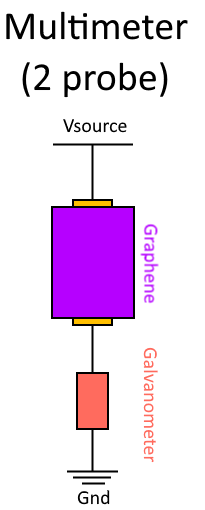
\includegraphics[width=\textwidth]{chap2/2probemeas}
			\caption{}\label{subfig:mutlimeter}
		\end{subfigure}\qquad
		\begin{subfigure}[t]{0.235\textwidth}
			\centering
			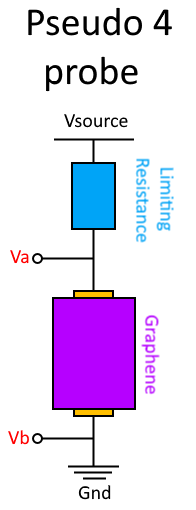
\includegraphics[width=\textwidth]{chap2/4probemeaspseudo}
			\caption{}\label{subfig:4probepseudo}
		\end{subfigure}\qquad
		\begin{subfigure}[t]{0.25\textwidth}
			\centering
			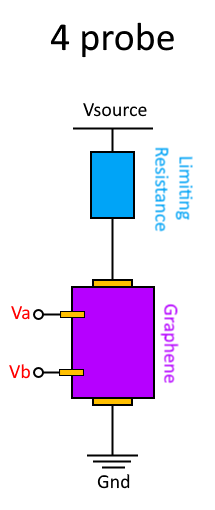
\includegraphics[width=\textwidth]{chap2/4probemeas}
			\caption{}\label{subfig:4probe}
		\end{subfigure}
		\caption[Schematics of resistance measurements]{Schematics of resistance measurements. (\subref*{subfig:mutlimeter}) A multimeter provides little control over the current through the sample, and measures any resistance formed between the gold contacts and the graphene. (\subref*{subfig:4probepseudo}) A pseudo 4 probe measurement uses a voltage difference across the device to calculate it's resistance, inclusive of the series resistance due to the gold contacts. (\subref*{subfig:4probe}) A 4 probe measurement uses a voltage difference measured by probes at different points on the sample material, thereby avoiding any contact resistance included in series, and sampling the voltage along the sample.}
		\label{fig:4probemeasurements}
	\end{figure}
	
	\subsubsection{Sourcemeters}
	
	A sourcemeter has the ability to source and measure a stable DC voltage or current. They provide precision, low noise and stability. We use Keithley 2400 SourceMeters \cite{keithley2400} which source voltage from $5\mu$V to 210V, and current from 50pA to 1.05A, and can deliver 520 readings per second at 5$\frac{1}{2}$ digits (ie, 199999).
	
	A source meter is used in 4 probe measurements to apply a constant, controlable gate voltage to the Si as directed in \cref{fig:instrumentation_device}. Changing the potential of Si under \silicondioxide{} changes the charged carrier density (electrons, holes) on graphene by using the \silicondioxide{} as a capacitor dielectric. This allows the measurement of the resistivity of graphene as a function of carrier density.
	
	\begin{figure}[H]
		\centering
		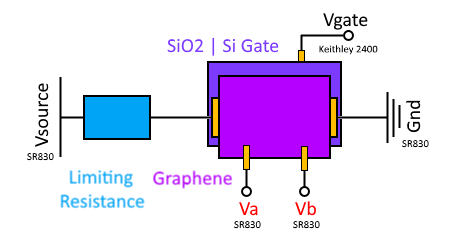
\includegraphics[width=0.6\textwidth]{chap2/4probemeasgated}
		\caption[Instrumentation connections to a gated graphene FET]{Instrumentation connections to a gated graphene FET,\\ using a Keithley 2400 SourceMeter and a SR830 Lock-In Amplifier.} \label{fig:instrumentation_device}
	\end{figure}
	
	\subsubsection{Lock-in amplifiers}
	A lock in amplifier is used to measure very small AC signals. This project used a Stanford Research 830 Lock-in amplifier\cite{sr830}, which uses a significant amount of digital dignal processing (DSP) for it's functionality. It operates on the principles of signal mixing - multiplying a input signal ($f_s$) that is expected at a particular frequency by a reference signal ($f_r$). This mixing generates a DC signal whose amplitude can be measured, directly inferring a signal strength. An example calculation of mixing is shown below in \cref{eqn:mixing}.
	
	\begin{align}
	f_{s}\otimes f_{r} &= \cos(\omega_{s} t + \phi) \otimes \cos(\omega_{r} t )\\
	&=	\left[\cos(\omega_{s} t)\cos(\phi) - \sin(\omega_{s}t)\sin(\phi)\right] \otimes \cos(\omega_{r} t )\nonumber\\
	&\begin{aligned}
		=&\cos(\phi)\frac{1}{2}\left[\cos\left(( \omega_s+  \omega_r)t\right) + \cos\left({( \omega_s - i \omega_r)t} \right)\right]\\
		&\hspace{0.5cm}-\sin(\phi)\frac{1}{2}\left[\sin\left((\omega_s + \omega_r)t\right)  + \sin\left((\omega_s - \omega_r)t\right)\right]
	\end{aligned}\label{eqn:mixing}
	\end{align}
	
	When the two frequencies $\omega_s$ and $\omega_r$ are close, then the sinsoidal components $\omega_s-\omega_r$ form a DC component, while high frequency compliment can be filtered. Only noise close to the signal frequency will be picked up in the filtering, and will only result in low frequency AC output. 
	
	The lock in amplifier uses a phase locked loop to generate a reference signal, which is a particular control circuit. The lock in amplifier can either run independently, generating it's own output, or can be locked to an external signal. We use the former in our measurements, to pass a slow 17Hz signal of amplitude 1V$_{rms}$ through graphene devices. 
	
	A voltage difference is calculated between probes on graphene by the lock in amplifier and outputted. The real component of the voltage difference and the complex phase are recorded - we expect the bulk transport in graphene to be resistive, and a phase is measured to confirm that as we measure.
	
	\subsection{Probe station}\label{sec:probestation}
	A LakeShore cryogenic probestation (\cref{fig:probestation}) was used to load sample wafers and measure their electronic properties under controlled conditions. In particular, we will touch on temperature control, vacuum ability, and the risk of static discharge.
		
	\begin{figure}[H]
		\centering
		\begin{tabular}[b]{cc}
			\multirow{2}{*}[1.5cm]{
				\centering
				\begin{subfigure}{0.55\textwidth}
					\centering
					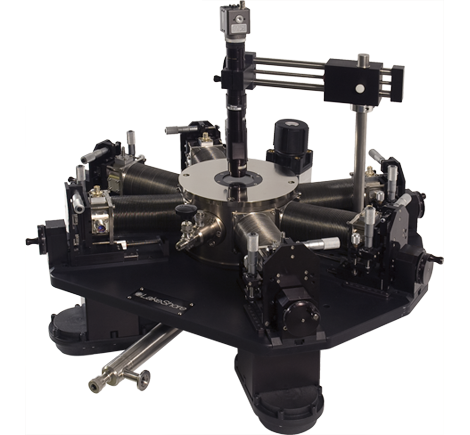
\includegraphics[width=\textwidth]{chap2/probestation}
					\caption{LakeShore probestation, with coolant inlet, 6 probe arms, vacuum seal and microscope camera.}
				\end{subfigure}
			}
			&\begin{subfigure}{0.4\textwidth}
				\centering
				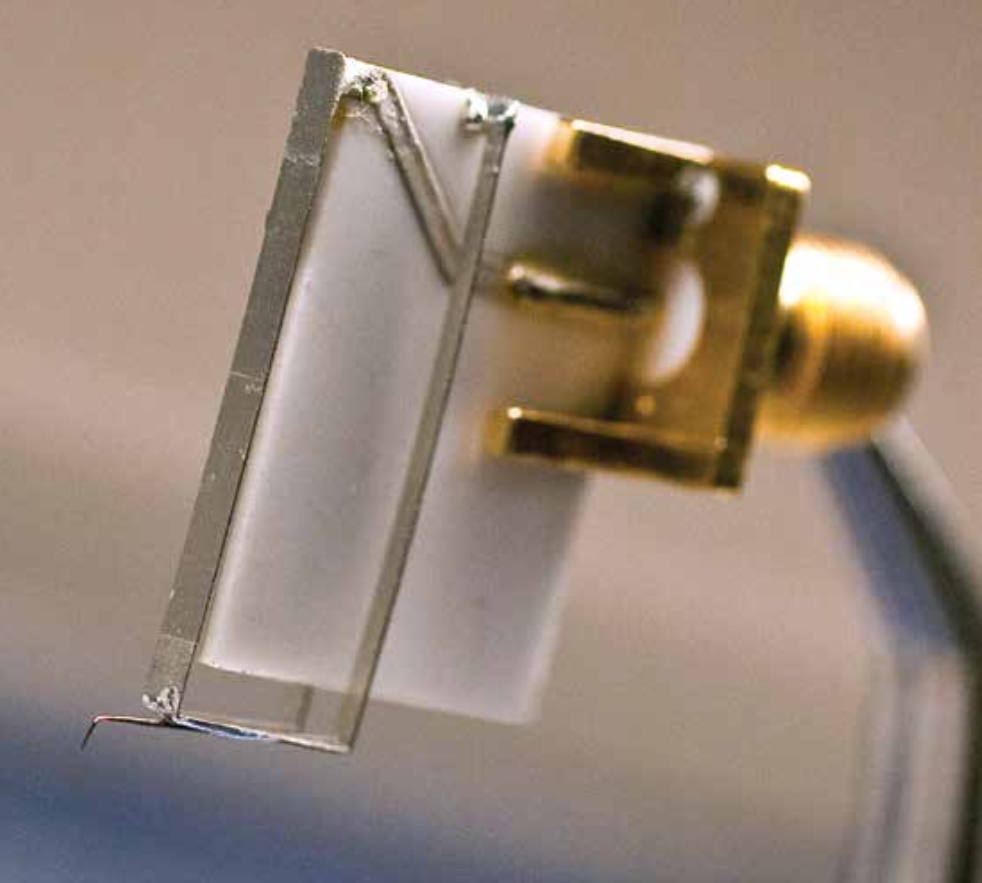
\includegraphics[width=0.8\textwidth]{chap2/probes}
				\caption{Tungsten spring probes, 25$\mu$m radius tip}
			\end{subfigure}\vspace{0.5cm}\\
			&\begin{subfigure}[b]{0.4\textwidth}
				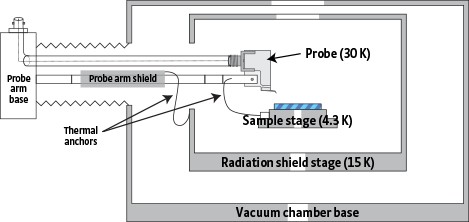
\includegraphics[width=\textwidth]{chap2/probestation_schem}
				\caption[Schematic diagram of probestation]{Schematic diagram of probestation, showing connections from probe arms to sample stage and temperature limits of elements}
			\end{subfigure}\\
		\end{tabular}
		\caption[LakeShore Probestation]{LakeShore probestation}\label{fig:probestation}
		%TODO Check that position is all correct - dodgy to setup...
	\end{figure}
	
	\subsubsection{Vacuum}
	A roughing pump is used in conjunction with a turbo pump to $1.5\times10^{-2}$bar and $7\times10^{-4}$bar (turbo). This pumping removes any trapped oxygen and contamination of gasses that might condense onto our sample of graphene at low temperature. 
	
	\subsubsection{Temperature control}
	To control the 
	
	\paragraph{PID control}
	\subsubsection{Static Discharge}
	\subsubsection{Probes}
	
	
\end{document}
	
	